% ! TEX root = ./introductory_thoughts.tex

\tikzset{every picture/.style={line width=0.75pt}} %set default line width to 0.75pt        

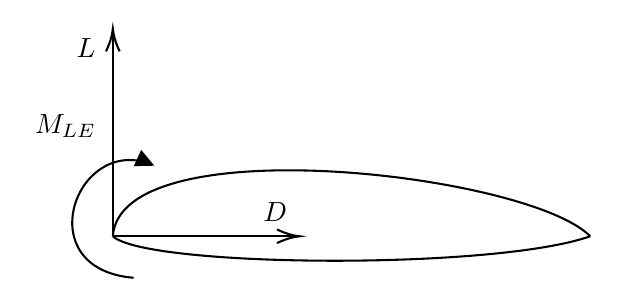
\begin{tikzpicture}[x=0.75pt,y=0.75pt,yscale=-1,xscale=1]
%uncomment if require: \path (0,300); %set diagram left start at 0, and has height of 300

%Curve Lines [id:da6282201102429681] 
\draw    (200,150) .. controls (203.67,97) and (400.18,119.75) .. (430,150) ;
%Curve Lines [id:da8779431608993546] 
\draw    (200,150) .. controls (216.34,165) and (383.51,166.41) .. (430,150) ;
%Straight Lines [id:da2590905789853304] 
\draw    (200,150) -- (200,52) ;
\draw [shift={(200,50)}, rotate = 90] [color={rgb, 255:red, 0; green, 0; blue, 0 }  ][line width=0.75]    (10.93,-3.29) .. controls (6.95,-1.4) and (3.31,-0.3) .. (0,0) .. controls (3.31,0.3) and (6.95,1.4) .. (10.93,3.29)   ;
%Straight Lines [id:da6275146811901227] 
\draw    (200,150) -- (288,150) ;
\draw [shift={(290,150)}, rotate = 180] [color={rgb, 255:red, 0; green, 0; blue, 0 }  ][line width=0.75]    (10.93,-3.29) .. controls (6.95,-1.4) and (3.31,-0.3) .. (0,0) .. controls (3.31,0.3) and (6.95,1.4) .. (10.93,3.29)   ;
%Curve Lines [id:da7637601528691369] 
\draw    (210,170) .. controls (159.47,165.85) and (181.66,102.38) .. (217.24,114.89) ;
\draw [shift={(220,116)}, rotate = 204.48] [fill={rgb, 255:red, 0; green, 0; blue, 0 }  ][line width=0.08]  [draw opacity=0] (8.93,-4.29) -- (0,0) -- (8.93,4.29) -- cycle    ;

% Text Node
\draw (181,53.4) node [anchor=north west][inner sep=0.75pt]    {$L$};
% Text Node
\draw (271,132.4) node [anchor=north west][inner sep=0.75pt]    {$D$};
% Text Node
\draw (161,90) node [anchor=north west][inner sep=0.75pt]    {$M_{LE}$};


\end{tikzpicture}
